In questo capitolo introdurremo due programmi fondamentali implementati con un'interfaccia a linea di comando, entrambi sviluppati con Python, che ci daranno la possibilità di interagire con il progetto realizzato.

\section{Cli}\label{capitolo_cli}
L'interfaccia a linea di comando Cli è uno strumento utile per poter richiedere informazioni sugli snapshot attraverso gli id forniti dal sistema centrale. Il codice del programma è presente al percorso \textit{sistema\_mobile/cli} nel file cli.py. Ogni sistema mobile avviato ha a disposizione un programma che gestisce un'interfaccia a linea di comando chiamata Cli attraverso il quale è possibile interfacciarsi al sistema mobile per poterlo interrogare. L'architettura del programma Cli è molto semplice: è stata implementata una connessione tra il sistema mobile e la Cli e tra il sistema mobile e il sistema centrale, sfruttando per entrambe le connessioni il protocollo TCP.

\subsection{Configurazione tra Cli e Sistema Mobile}
Per avviare correttamente il nuovo sistema di certificazione realizzato, è necessario configurare la comunicazione TCP tra la componente sistema mobile e il programma Cli. Operazione realizzata attraverso la semplice modifica di due variabili presenti sia nel file Python sistemamobile.py, contenuto nella cartella \textit{sistema\_mobile} che nel file cli.py, contenuto nel percorso \textit{sistema\_mobile/cli}. Per comodità, le due variabili presenti nei due file assumono lo stesso nome: host\_cli e port\_cli. E' doveroso ribadire anche se evidente, che la variabile host\_cli oltre a contenere un indirizzo host valido dovrà apparire con lo stesso valore in entrambi i file e la stessa considerazione varrà anche per port\_cli anche se in questa circostanza dovrà invece contenere un numero di porta valido.
\subsection{Autenticazione degli id}\label{autenticazionedegliid}
\begin{figure}[!h]
\centering
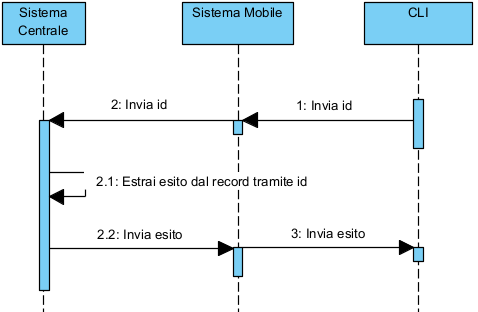
\includegraphics[scale=0.9]{images/Richiesta autenticazione id.png}
\caption{Richiesta autenticazione di un id}
\label{fig: richiesta_autenticazione_id }
\end{figure}
Il sistema centrale come già sappiamo, confronta lo snapshot ricevuto dal sistema mobile con quello ricevuto dalla stazione di riferimento, calcola l'identificatore (o id) associato allo snapshot ricevuto dal sistema mobile sfruttando una funzione hash\footnote{La funzione hash utilizzata è la sha\_256 e viene applicata allo snapshot ricevuto dal sistema mobile.}, e infine lo invia a quest'ultimo. E' attraverso questo id che il sistema mobile può richiedere l'esito dell'autenticazione dello snapshot oltre ad altre informazioni. Per richiedere l'autenticazione degli id si sfrutta il comando \textit{verifica\_id <id>}. L'implementazione avviene con una comunicazione TCP tra la Cli e il sistema mobile che a sua volta comunicherà con il sistema centrale, il quale ci restituirà un valore booleano [vedi figura \ref{fig: richiesta_autenticazione_id }]. Il valore booleano restituito sarà True se l'id associato allo snapshot è stato autenticato correttamente, False altrimenti. Una risposta negativa ci fa intendere che lo snapshot associato all'id da verificare è stato corrotto. Qualche malintenzionato ha quindi interferito con il ricevitore satellitare del sistema mobile facendo sì che il segnale non fosse catturato dai satelliti, ma da un terzo dispositivo che inviava dati manipolati. In figura \ref{fig: verifica_id } mostriamo un esempio di utilizzo del comando \textit{verifica\_id}.
\begin{figure}[!h]
\centering
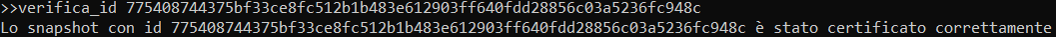
\includegraphics[scale=0.8]{images/verifica_id.png}
\caption{Un esempio di utilizzo del comando verifica\_id}
\label{fig: verifica_id }
\end{figure}

\subsection{Stampa lista degli id}
Attraverso il comando \textit{stampa\_lista\_id} è possibile richiedere tutti gli id inviati dal sistema centrale al sistema mobile fino a quel momento. Ogni volta che il sistema mobile riceve un id dal sistema centrale lo memorizza all'interno del file id\_list.json, in questo modo manterrò la persistenza degli id e quando dal programma Cli voglio ottenerli, sarà sufficiente inviare una richiesta al sistema mobile che inoltrerà l'intera lista. Nella figura \ref{fig: stampalistaid } mostriamo un esempio di utilizzo del comando.
\begin{figure}[!h]
\centering
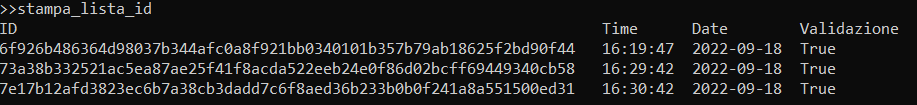
\includegraphics[scale=0.8]{images/stampa_lista_id.png}
\caption{Un esempio di utilizzo del comando stampa\_lista\_id}
\label{fig: stampalistaid }
\end{figure}

\subsection{Info posizione a partire da un id}
La procedura di richiesta delle informazioni di posizione a partire da un id, avviene con il comando \textit{info\_id <id>}, che si comporta in maniera molto simile alla procedura di richiesta dell'esito dell'autenticazione degli snapshot vista sopra [vedi sottosezione \ref{autenticazionedegliid}]. Il primo messaggio viene inviato dalla Cli e rappresenta una stringa che contiene il comando "info\_id", per far capire al sistema mobile il tipo di operazione da svolgere. Ricevuta la conferma di ricezione del messaggio può inviare l'id da verificare. Il sistema mobile, dopo aver ricevuto questi due messaggi può comunicare con il sistema centrale, il quale, dopo aver ricevuto l'id sfrutta il file metadati.json. In tal modo ottiene il file dei metadati associato a quell'identificatore (id) per estrarre le informazioni di posizione da inviare al sistema mobile per poi essere inoltrate alla Cli. Per chiarire meglio le idee è possibile visionare il diagramma di sequenza in figura \ref{fig: informazioni_id } che spiega lo scambio di messaggi step by step. Nella figura \ref{fig: info_id2 } vediamo invece un esempio di utilizzo del comando \textit{info\_id}.
\begin{figure}[!h]
\centering
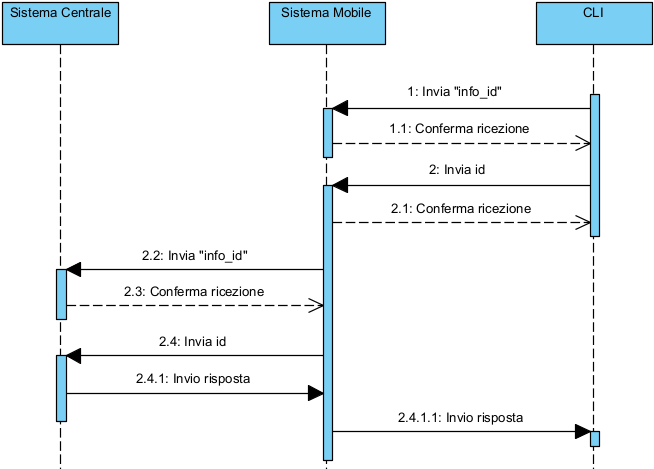
\includegraphics[scale=0.8]{images/info_id.png}
\caption{Diagramma per descrivere la comunicazione tra componenti per la realizzazione del comando info\_id}
\label{fig: informazioni_id }
\end{figure}
\begin{figure}[!h]
\centering
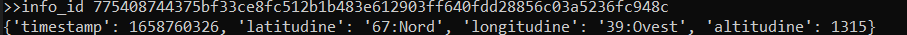
\includegraphics[scale=0.8]{images/info_id2.png}
\caption{Un esempio di utilizzo del comando info\_id}
\label{fig: info_id2 }
\end{figure}

\subsection{Altri comandi}
Vediamo gli altri comandi disponibili con l'interfaccia a linea di comando Intecs.
\begin{itemize}
    \item \textit{help}: restituisce la lista di tutti i comandi disponibili con una piccola didascalia per rendere più chiaro il funzionamento di ognuno di questi.
    \item \textit{clear}: ripulisce la schermata del programma cancellando ogni scritta presente.
    \item \textit{exit}: viene usato per chiudere correttamente il programma.
\end{itemize}

\subsection{Tabella riassuntiva dei comandi}
\scalebox{0.9}{
\begin{tabular}{llllll}
\toprule
{\bfseries Comando} & {\bfseries Sintassi} & {\bfseries
Esempio}\\
\midrule
stampa\_lista\_id & stampa\_lista\_id  & stampa\_lista\_id \\
\midrule
verifica\_id & verifica\_id <id> & verifica\_id 597c28c381ef1fee \\
\midrule
info\_id & info\_id <id> & info\_id 597c28c381ef1fee \\
\midrule
help & help & help \\
\midrule
exit & exit & exit \\
\midrule
clear & clear & clear \\
\bottomrule
\end{tabular}}

% \hspace{-1.7 cm}
% \begin{center}
% \centering
% \begin{tabular}{|l|c|c|}
% \hline
% \multicolumn{3}{|c|}{}\\
% \multicolumn{3}{|c|}{\textbf{\Large Comandi}}\\
% \multicolumn{3}{|c|}{}\\
% \hline
% \multicolumn{1}{|c|}{\textbf{Comando}} & \textbf{Sintassi} &
% \multicolumn{1}{c|}{\textbf{Esempio}}\\
% \hline
% stampa\_lista\_id & stampa\_lista\_id  & stampa\_lista\_id \\
% verifica\_id & verifica\_id <id> & verifica\_id 597c28c381ef1fee \\
% info\_id & info\_id <id> & info\_id 597c28c381ef1fee \\
% help & help & help \\
% exit & exit & exit \\
% clear & clear & clear \\
% \hline
% \end{tabular}
% \end{center}

\section{Cli v2}
Sono state implementate due versioni del programma Cli implementato con un'interfaccia a linea di comando. La prima versione comunica con il sistema mobile per richiedere le informazioni degli snapshot ed è stata approfondita poco fa. In questa seconda versione invece, il programma si interfaccia direttamente con la blockchain comunicando attraverso l'Indexer V2 (approfondito nel capitolo \ref{2.statoarte}). Il codice del programma è presente al percorso \textit{sistema\_mobile/'cli v2'} nel file cli.py. Prima di poter avviare questo file Python è necessario configurare il file config.json in maniera corretta. Nel codice seguente mostriamo un fac-simile del contenuto dove \textit{indirizzo pubblico} dovrà essere sostituito con il valore dell'indirizzo pubblico Algorand del sistema centrale.
\lstinputlisting[label= cod: config1cli2, caption= esempio del contenuto nel file config.json, language=json, basicstyle=\small]{listing/sourceCode/configjson_cliv2.json}
L'implementazione di questa versione del programma è molto semplice: si estraggono le transazioni dalla blockchain il cui mittente è l'indirizzo Algorand del sistema centrale attraverso il metodo \textit{search\_transaction\_by\_address(address)} fornito dall'Indexer di Algorand. Le transazioni restituite saranno quelle riferite ai metodi \textit{compare\_hash()} e \textit{validate\_snapshot()} ma visto che ci interessa il  contenuto del campo nota utilizzeremo solo le transazioni di \textit{validate\_snapshot()}. Nella figura \ref{fig: camponota } mostriamo il campo nota  di una transazione riferita al metodo \textit{validate\_snapshot()} attraverso AlgoExplorer\footnote{AlgoExplorer è una piattaforma che consente di esplorare e cercare nella blockchain di Algorand transazioni, indirizzi, statistiche, smart contract e altro ancora.} \cite{algoexplorer}. Notiamo subito, che il campo nota è formato dai seguenti parametri:
\begin{itemize}
    \item account\_address\_sistema\_mobile: ci indica quale account Algorand del sistema mobile ha ricevuto lo snapshot in questione.
    \item id: rappresenta l'identificatore (id) univoco allo snapshot restituitoci dal sistema centrale.
    \item hash\_snapshot\_sm: rappresenta l'hash calcolato con la funzione sha\_256 dello snapshot.
    \item timestamp: rappresenta la data e l'ora in cui il sistema mobile ha ricevuto lo snapshot dalla componente antenna.
    \item latitudine, longitudine, altitudine: rappresentano dati di posizione che si riferiscono alla posizione in cui si trovava il sistema mobile al momento dell'acquisizione dei segnali da antenna.
\end{itemize}
\begin{figure}[!h]
\centering
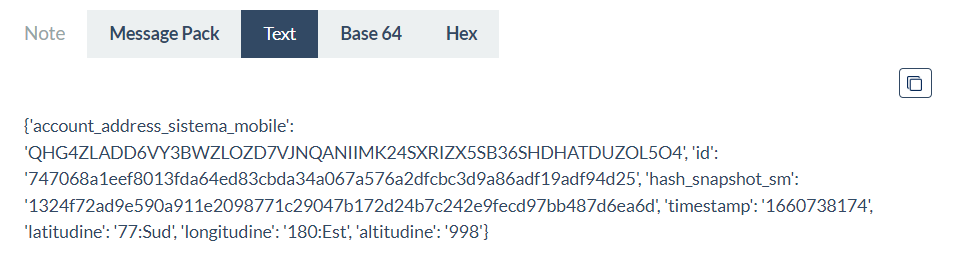
\includegraphics[scale=0.8]{images/campo_nota.png}
\caption{Un esempio del campo nota della transazione riferita al metodo validate\_snapshot()}
\label{fig: camponota }
\end{figure}
Di seguito approfondiamo l'implementazione dei comandi del programma Cli v2.

\subsection{Stampa lista degli id}\label{stampalistaid}
Il comando \textit{stampa\_lista\_id} restituisce gli id (o identificatori) inviati dal sistema centrale al sistema mobile fino a quel momento, ma non tutti, infatti ci restituisce solamente quelli il cui snapshot ha riportato un esito positivo nella certificazione. Questo per il semplice fatto che se un id associato ad uno snapshot non supera la fase di autenticazione, non sarà richiamato il metodo \textit{validate\_snapshot()} per questo snapshot e di conseguenza non compariranno in blockchain le sue informazioni. La ricerca degli id si effettua anche in questo caso, con il metodo \textit{search\_transaction\_by\_address()}, il cui argomento sarà sempre l'indirizzo Algorand del sistema centrale. Questo metodo ci restituirà una lista contenente tutte le transazioni in cui il mittente è il sistema centrale. Dovremo anche in questo caso filtrare le transazioni ed estrarre solo quelle riferite al metodo \textit{validate\_snapshot()}. Dunque, estrarremo da ognuna di queste transazioni il campo nota e da quest'ultimo acquisiremo l'id. Attraverso quest'implementazione potremo ottenere quindi, ogni id.

\subsection{Autenticazione degli id}
Il comando \textit{verifica\_id <id>} estrae la lista degli id come abbiamo visto con il comando \textit{stampa\_lista\_id} (vedi sottosezione \ref{stampalistaid}), prendendo quindi il campo id di ogni transazione e confrontandolo con il campo <id> passato per argomento. Lo scopo è di trovare la transazione il cui id corrisponde a quello passato per argomento. Se si verifica questa condizione, posso dire con certezza che lo snapshot associato a tale id è stato autenticato correttamente. Ribadiamo che gli snapshot che non superano la fase di confronto e non vengono quindi certificati, non saranno caricati sulla blockchain con la transazione riferita al metodo \textit{validate\_snapshot()}.

\subsection{Info posizione a partire da un id}
Il comando \textit{info\_id <id>} estrae il campo noto dalle transazioni riferite al metodo \textit{validate\_snapshot}, cerca la transazione il cui campo nota ha come id quello passato per argomento ed estrae i dati di posizione (latitudine, longitudine, altitudine) ed il timestamp di quel campo nota.

\subsection{Settaggio dell'indirizzo Algorand di Sistema Centrale}
Il comando \textit{set\_address\_sistemacentrale <address>} si utilizza per impostare il valore di sistema\_centrale\_address del file config.json attraverso il quale possiamo settare l'account Algorand di cui restituiremo le transazioni, tramite l'utilizzo del metodo dell'Indexer \textit{search\_transaction\_by\_address()}.

\subsection{Altri comandi}
Vediamo gli altri comandi disponibili con il programma Intecs.
\begin{itemize}
    \item \textit{help}: restituisce la lista di tutti i comandi disponibili con una piccola didascalia per rendere più chiaro il funzionamento di ognuno di questi.
    \item \textit{clear}: ripulisce la schermata del programma cancellando ogni scritta presente.
    \item \textit{exit}: viene usato per chiudere correttamente il programma.
\end{itemize}

\subsection{Tabella riassuntiva dei comandi}
\resizebox{\textwidth}{!}{%
\begin{tabular}{llllll}
\toprule
{\bfseries Comando} & {\bfseries Sintassi} & {\bfseries
Esempio}\\
\midrule
stampa\_lista\_id & stampa\_lista\_id  & stampa\_lista\_id \\
\midrule
verifica\_id & verifica\_id <id> & verifica\_id 597c28c381ef1fee \\
\midrule
info\_id & info\_id <id> & info\_id 597c28c381ef1fee \\
\midrule
set\_address\_sistemacentrale & set\_address\_sistemacentrale <address> & set\_address\_sistemacentrale 597c28c381ef1fee \\
\midrule
help & help & help \\
\midrule
exit & exit & exit \\
\midrule
clear & clear & clear \\
\bottomrule
\end{tabular}}

\section{Intecs}
Lo smart contract viene creato e gestito da Intecs SpA attraverso il programma Intecs, implementato con un'interfaccia a linea di comando per permettere alcune operazioni critiche come la creazione ed eliminazione degli smart contract. Il codice Python del programma Intecs è presente nella cartella \textit{intecs} nel file intecs.py e rappresenta proprio il programma da dover avviare per far funzionare l'interfaccia a linea di comando in questione.

\subsection{File di configurazione}
Nella cartella \textit{intecs}, oltre al file intecs.py si trova il file config.json al cui interno ha i parametri fondamentali per potersi collegare alla blockchain e allo smart contract. 
\lstinputlisting[label= cod: request, caption= esempio del contenuto nel file config.json, language=json, basicstyle=\small]{listing/sourceCode/config_intecs.json}
Contiene infatti, l'indice dello smart contract (app id) creato e l'indirizzo Algorand del sistema centrale.

\subsection{Il primo avvio del programma}
Al primo avvio del programma intecs.py viene ricordato di creare gli account Algorand, senza i quali non sarebbe possibile creare lo smart contract né tantomeno interagirci. Nella figura \ref{fig: intecs_primoavvio_ } mostriamo l'interfaccia al primo avvio dove in questo particolare esempio viene digitato da tastiera la stringa "NO" che non darà modo di creare lo smart contract.
% \begin{figure}[!h]
% \flushleft
% 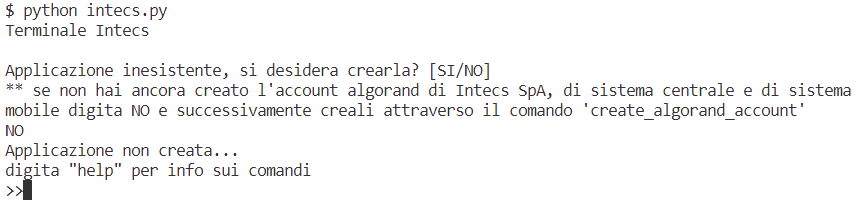
\includegraphics[scale=0.8]{images/Intecs/primo_avvio.png}
% \caption{Primo avvio dell'applicazione}
% \label{fig: intecs_primoavvio_ }
% \end{figure}
Il messaggio "Applicazione inesistente, si desidera crearla? [SI/NO]" viene mostrato ad ogni avvio finché lo smart contract  non verrà creato.
 
\subsection{Generare un account Algorand}\label{generareaccountalgorand}
La creazione di un account Algorand sulla rete TestNet è una procedura molto semplice utilizzando il programma Intecs, ci basta digitare il comando \textit{create\_algorand\_account} [vedi figura \ref{fig: intecs_create_algorand_account}].
\begin{figure}[!h]
\flushleft
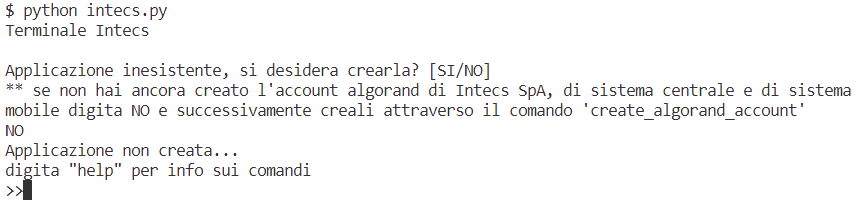
\includegraphics[scale=0.8]{images/Intecs/primo_avvio.png}
\caption{Primo avvio dell'applicazione}
\label{fig: intecs_primoavvio_ }
\end{figure}
\begin{figure}[!h]
\centering
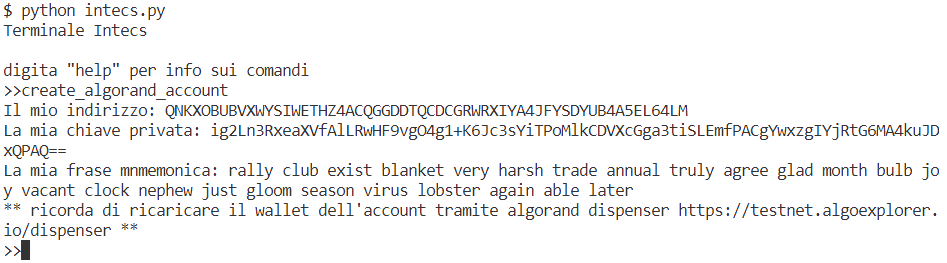
\includegraphics[scale=0.8]{images/Intecs/create_algorand_account.png}
\caption{Creazione di un Algorand account tramite l'interfaccia a linea di comando Intecs}
\label{fig: intecs_create_algorand_account}
\end{figure}\\
Una volta creato l'account, è necessario memorizzare manualmente i tre campi restituiti. Come viene suggerito anche nella fase di creazione dell'account dal programma Intecs, devono essere aggiunti Algos nel Wallet dell'account attraverso l'Algorand Dispenser \cite{algoranddispenser}.

\subsection{Creazione dello smart contract}\label{creazione_smart_contract}
Lo smart contract è un contratto che è possibile creare solamente dopo la creazione dell'account Algorand di Intecs SpA. Successivamente è necessario modificare i valori delle tre variabili globali (intecs\_address, intecs\_privatekey e intecs\_passphrase) del programma intecs.py che si trovano sotto la dichiarazione delle librerie, nelle prime righe del codice. Dopo questa procedura, bisogna creare anche l'account associato al sistema centrale. La figura \ref{fig: intecs_create_smart_contract_} mostra il programma Intecs nella fase di creazione dello smart contract, al termine del quale restituirà l'application-id, un identificatore univoco. Con la creazione dello smart contract è necessario come suggerito anche dall'interfaccia a linea di comando Intecs, settare manualmente l'app-id di sistema centrale, di sistema mobile nei due file config.json, che si trovano rispettivamente nella cartella \textit{sistema\_centrale} e \textit{sistema\_mobile}. La fase di opt-in dell'account Intecs è cruciale perché imposta il valore della variabile globale address\_sistema\_centrale dello smart contract appena creato. La condizione necessaria affinché la creazione di una nuova app vada a buon fine è che l'app corrente sia stata eliminata o che si tratti del primo avvio del programma. In questo modo si evita di avere duplicati di smart contract associati all'account Algorand di Intecs.
\begin{figure}[!h]
\centering
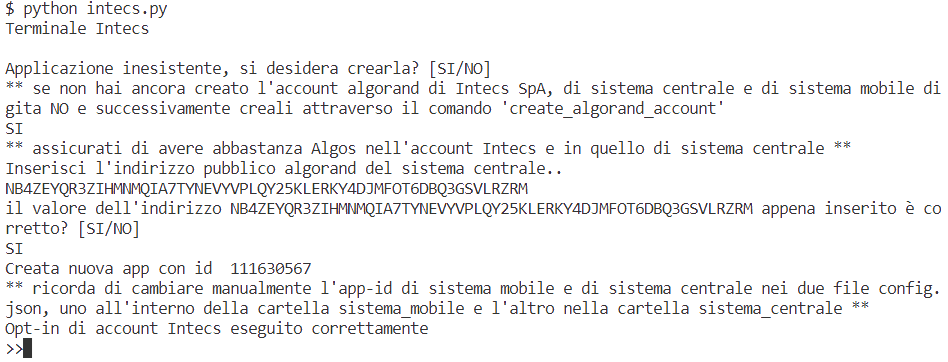
\includegraphics[scale=0.8]{images/Intecs/creazione_smartcontract.png}
\caption{Creazione dello smart contract}
\label{fig: intecs_create_smart_contract_}
\end{figure}

\subsection{Eliminazione dello smart contract}
Il comando \textit{delete\_app} [vedi figura \ref{fig: intecs_delete_smart_contract}] elimina lo smart contract corrente se e solo se il valore di app\_id nel file config.json risulta diverso da 0 e cioè se e solo se esiste. Attraverso il metodo ApplicationDeleteTxn che effettua una transazione alla blockchain si eliminerà lo smart contract. Dopo l'eliminazione sarà di nuovo possibile crearlo con il comando \textit{create\_app} visto nella sezione \ref{creazione_smart_contract}.
\begin{figure}[!h]
\flushleft
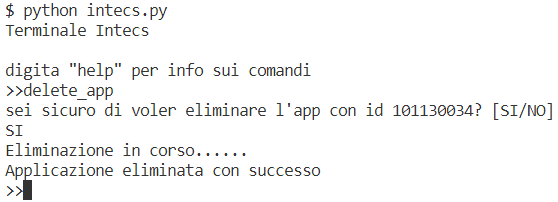
\includegraphics[scale=0.8]{images/Intecs/eliminazione_app.png}
\caption{Eliminazione dello smart contract}
\label{fig: intecs_delete_smart_contract}
\end{figure}

\subsection{Altri comandi}
Vediamo gli altri comandi disponibili con l'interfaccia a linea di comando Intecs.
\begin{itemize}
    \item \textit{app-id}: restituisce l'indice (app-id) univoco associato allo smart contract. Il funzionamento è semplice: si legge il valore della chiave 'app\_id' nel file config.json e si restituisce. Se il valore è impostato a 0 significa che l'applicazione non è mai stata creata oppure è stata eliminata e non è quindi più esistente.
    \item \textit{set\_account\_sistemacentrale}: serve per cambiare il valore della variabile globale address\_sistema\_centrale dello smart contract e di sistema\_centrale\_address nel file config.json. La procedura di modifica può essere eseguita esclusivamente dall'account Algorand di Intecs.
    \item \textit{address\_sistemacentrale}: restituisce, se esiste, il valore dell'indirizzo Algorand del sistema centrale. Semplicemente si effettua una lettura del valore della chiave "sistema\_centrale\_address" nel file config.json per poi restituirla; se il valore è impostato su stringa vuota ("") significa che l'applicazione non è mai stata creata.
    \item \textit{exit}: comando usato per chiudere correttamente il programma.
    \item \textit{clear}: ripulisce la schermata del programma cancellando ogni scritta presente.
    \item \textit{help}: restituisce la lista di tutti i comandi disponibili con una piccola didascalia per rendere più chiaro il funzionamento di ognuno di questi.
\end{itemize}

\subsection{Tabella riassuntiva dei comandi}
\resizebox{\textwidth}{!}{%
\begin{tabular}{llllll}
\toprule
{\bfseries Comando} & {\bfseries Sintassi} & {\bfseries
Esempio}\\
\midrule
create\_app & create\_app & create\_app \\
\midrule
app-id & app-id & app-id \\
\midrule
delete\_app & delete\_app & delete\_app \\
\midrule
set\_account\_sistemacentrale & set\_account\_sistemacentrale <address> & set\_account\_sistemacentrale 597c28c381ef1fee \\
\midrule
create\_algorand\_account & create\_algorand\_account & create\_algorand\_account \\
\midrule
address\_sistemacentrale & address\_sistemacentrale & address\_sistemacentrale \\
\midrule
exit & exit & exit \\
\midrule
clear & clear & clear \\
\bottomrule
\end{tabular}}
